\def\assignmenttitle{Estimating the Trajectory of a Satellite}
\def\assignmentnumber{5}
\def\assignmentdate{02-12-2011}
\def\githuburl{\small\url{https://github.com/alphabits/dtu-fall-2011/tree/master/02417/assignment-5}}
\def\githuburlfoot{\footnotesize\url{https://github.com/alphabits/dtu-fall-2011/tree/master/02417/assignment-5}}

\def\myepsilon{\varepsilon}
\def\erm{\myepsilon_{rt}}
\def\etm{\myepsilon_{\theta t}}
\def\erp{\myepsilon^p_{rt}}
\def\etp{\myepsilon^p_{\theta t}}
\def\evp{\myepsilon^p_{v_\theta t}}
\def\vecX{\myvec{X}}
\def\vecYt{\myvec{Y}_t}
\def\vece{\myvec{e}}
\def\vecSigma{\myvec{\Sigma}}
\def\vecA{\myvec{A}}
\def\vecC{\myvec{C}}


\documentclass[11pt]{article}
\linespread{1}

\renewcommand{\thefootnote}{\fnsymbol{footnote}}

\usepackage{geometry} % see geometry.pdf on how to lay out the page. There's lots.
\usepackage[utf8]{inputenc}
\usepackage[T1]{fontenc}
\usepackage{array}
\usepackage{amsmath,amssymb,latexsym,epic,eepic,epsfig,graphics,psfrag}
\usepackage{amsfonts}
\usepackage{graphicx,float}
\usepackage{color}
\definecolor{mygray}{RGB}{244,244,244}
\definecolor{gray}{gray}{0.5}
\definecolor{myredish}{RGB}{193,33,97}
\definecolor{grayblue}{RGB}{91,112,142}
\definecolor{myorange}{RGB}{255,134,0}
\definecolor{green}{rgb}{0,0.4,0}

\usepackage[english]{babel}

\usepackage[bottom]{footmisc}

\usepackage{fancyhdr}
\pagestyle{fancy}
\lhead{\small\textit{Assignment \assignmentnumber -- 02417 Time Series Analysis -- Anders Hørsted (s082382)}}
\rhead{\thepage}
\chead{}
\lfoot{}\cfoot{}\rfoot{}

\usepackage{subfigure}
\usepackage{pstricks}
\usepackage{pst-node}
\usepackage{wrapfig}
\usepackage{caption}
\usepackage{multirow}
%\usepackage{fouriernc}
%\usepackage[charter]{mathdesign}
\usepackage{lmodern}
\usepackage[normalem]{ulem}
\geometry{a4paper} % or letter or a5paper or ... etc
% \geometry{landscape} % rotated page geometry

\usepackage{url}


\makeatletter
\renewcommand*\env@matrix[1][*\c@MaxMatrixCols c]{%
  \hskip -\arraycolsep
  \let\@ifnextchar\new@ifnextchar
  \array{#1}}
\makeatother

\newcommand\myimp{\quad\Leftrightarrow\quad}
\newcommand\half{\frac{1}{2}}
\newcommand\myvec[1]{\mathbf{#1}}
\newcommand\mymod[1]{\ (\text{mod }#1)}
\newcommand\myreal{\mathbb{R}}
\newcommand\mynatural{\mathbb{N}}
\newcommand\myinteger{\mathbb{Z}}
\newcommand\mycomplex{\mathbb{C}}
\newcommand\myint{\text{int}}
\newcommand\norm[1]{||\,#1\,||}
\newcommand\bignorm[1]{\big|\big|\,#1\,\big|\big|}
\newcommand\seq[1]{\big\{#1\big\}}
\newcommand\smallseq[1]{\{#1\}}
\newcommand\smallseqtoinf[1]{\smallseq{#1}_{k=1}^\infty}
\newcommand\lonew{\ell^1_w}
\newcommand\lone{\ell^1}
\newcommand\ltwo{\ell^2(\mynatural)}
\newcommand\ip[2]{\langle#1,#2\rangle}
\newcommand\hilbert[1]{\mathcal{#1}}
\newcommand\uinf{u_{\infty}}
\newcommand\erf{\text{erf\,}}
\newcommand\infint{\int_{\infty}^{\infty}}
\newcommand\fpi{FPI}
\newcommand\E[1]{\text{E}[#1]}
\newcommand\Var[1]{\text{Var}[#1]}
\newcommand\Cov[1]{\text{Cov}[#1]}
\newcommand\myverb[1]{{\footnotesize\texttt{#1}}}
\newcommand\Yhat{\widehat{Y}}
\newcommand\given{\,|\,}

\usepackage[scaled]{beramono}
\usepackage{listings}
\lstset {                 % A rudimentary config that shows off some features.
    language=R,
    basicstyle=\scriptsize\ttfamily, % Without beramono, we'd get cmtt, the teletype font.
    commentstyle=\textit, % cmtt doesn't do italics. It might do slanted text though.
    keywordstyle=,
    identifierstyle=,
    framextopmargin=4pt,
    framexbottommargin=4pt,
    framexleftmargin=4pt,
    framexrightmargin=4pt,
    xleftmargin=4pt,
    xrightmargin=4pt,
    backgroundcolor=\color{mygray},
    frame=single,
    showstringspaces=false,
    captionpos=b,
    tabsize=4            % Or whatever you use in your editor, I suppose.
}

\renewcommand{\lstlistlistingname}{Code Listings}
\renewcommand{\lstlistingname}{Code Listing}

\usepackage{tabulary}
\newcolumntype{y}{>{\centering\arraybackslash}R}

\title{\assignmenttitle}
\date{\assignmentdate}
\author{Assignment \assignmentnumber\ -- 02417 Time Series Analysis -- Anders Hørsted (s082382)}
%\author{}
\date{} % delete this line to display the current date



%%% BEGIN DOCUMENT
\begin{document}

\maketitle

In this report the trajectory of an orbiting satellite will be reconstructed and predicted, based on 50 measurements $\{(r_t^m, \theta_t^m)\}_{t=1}^{50}$ of the position of the satellite given in polar coordinates. Due to imprecision in the measurement process, the real position of the satellite $(r_t^p, \theta_t^p)$ is related to the measurements by
\begin{align*}
    r_t^m &= r_t^p + \erm \\
    \theta_t^m &= \theta_t^p + \etm
\end{align*}
where $\erm\sim N(0,2000^2)$, $\etm\sim N(0,0.03^2)$ and $\erm$, $\etm$ are independent.

\section*{Formulating a model}
To reconstruct and predict the trajectory of the satellite, we will create a state space model. The state vector is defined as
\begin{equation*}
    \vecX_t = \begin{pmatrix}
        r^p_t \\
        \theta^p_t \\
        v^p_{\theta t}
    \end{pmatrix}
\end{equation*}
where $r^p_{t}$ is the true distance to the satellite, $\theta^p_t$ is the angle, and $v^p_{\theta t}$ is the angle velocity. It is assumed that the trajectory is well approximated by a circle, but to include deviations from a perfect circle, we define the random deviations
\begin{equation*}
    \erp \sim N(0,500^2), \quad \etp\sim N(0,0.005^2), \quad \evp \sim N(0, 0.005^2)
\end{equation*}
and then model the dynamics of the state vector, by the equations
\begin{align*}
    r^p_t &= r^p_{t-1} + \erp \\
    \theta^p_t &= \theta^p_{t-1} + v^p_{t-1} + \etp \\
    v^p_t &= v^p_{t-1} + \evp
\end{align*}
\todo{Comment on model formulation!!!}
To write the state space model on matrix form, we define the measurement vector by
\begin{equation*}
    \vecYt = \begin{pmatrix}
        r^m_t \\
        \theta^m_t
    \end{pmatrix}
\end{equation*}
and two random vectors by
\begin{equation*}
    \vece_1 = \begin{pmatrix}
        \erp \\
        \etp \\
        \evp
    \end{pmatrix}, \quad \vece_2 = \begin{pmatrix}
        \erm \\
        \etm
    \end{pmatrix}
\end{equation*}
Since $\erp,\etp$ and $\evp$ are independent, and also $\erm$ and $\etm$ are independent
\begin{equation*}
    \vecSigma_1 = \Var{\vece_1} = \begin{bmatrix}
        500^2 & 0 & 0 \\
        0 & 0.005^2 & 0 \\
        0 & 0 & 0.005^2
    \end{bmatrix}, \quad \vecSigma_2 = \Var{\vece_2} = \begin{bmatrix}
        2000^2 & 0 \\
        0 & 0.03^2
    \end{bmatrix}
\end{equation*}
By setting
\begin{equation*}
    \vecA = \begin{bmatrix}
        1 & 0 & 0 \\
        0 & 1 & 1 \\
        0 & 0 & 1
    \end{bmatrix}, \quad \vecC = \begin{bmatrix}
        1 & 0 & 0 \\
        0 & 1 & 0
    \end{bmatrix}
\end{equation*}
the state space model can now be expressed by the system equation
\begin{equation*}
    \vecX_t = \vecA\vecX_{t-1} + \vece_1
\end{equation*}
and the observation equation
\begin{equation*}
    \vecYt = \vecC\vecX_t + \vece_2
\end{equation*}

Using the defined model the trajectory can now be reconstructed and predicted by using the Kalman filter. To actually use the Kalman filter, it needs to be implemented.

\section*{Implementing the Kalman filter}
In this section the Kalman filter is implemented in R. The implementation (see listing~\ref{lst:kalman}) is a regular R script that first loads the data in the variable \myverb{dat}

\vspace{3mm}
\lstinputlisting[caption={Implementation of the Kalman filter},label=lst:kalman]{../src/kalman.R}


\section*{Reconstructing the trajectory}
In this section the implementation of the Kalman filter is used to reconstruct the trajectory of the satellite.

\begin{figure}[ht]
    \centering
    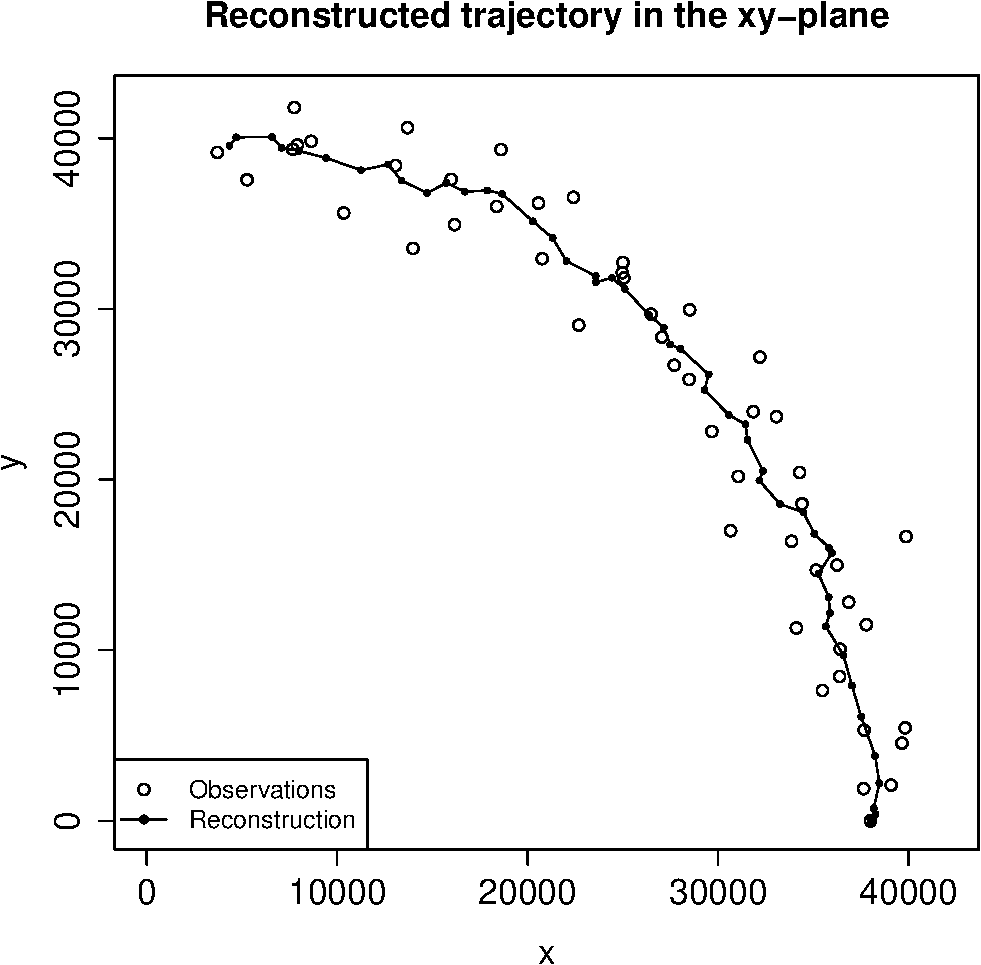
\includegraphics[width=70mm]{../plots/reconstruction.pdf}
    \caption{CAPTION XXX}
    \label{fig:reconstruction}
\end{figure}

\section*{Predicting the trajectory}

\begin{figure}[ht]
    \centering
    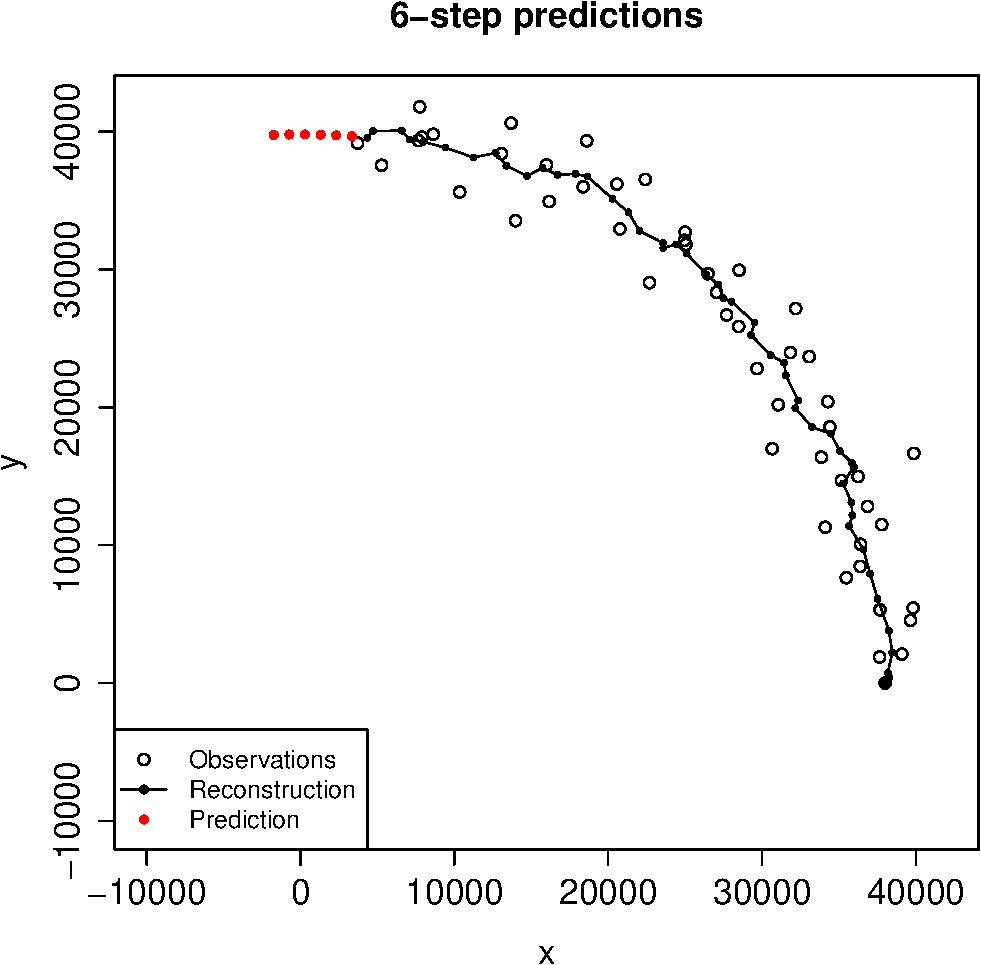
\includegraphics[width=70mm]{../plots/all-predictions.pdf}
    \caption{CAPTION XXX}
    \label{fig:all-predictions}
\end{figure}

\begin{figure}
    \centering
    \mbox{\subfigure{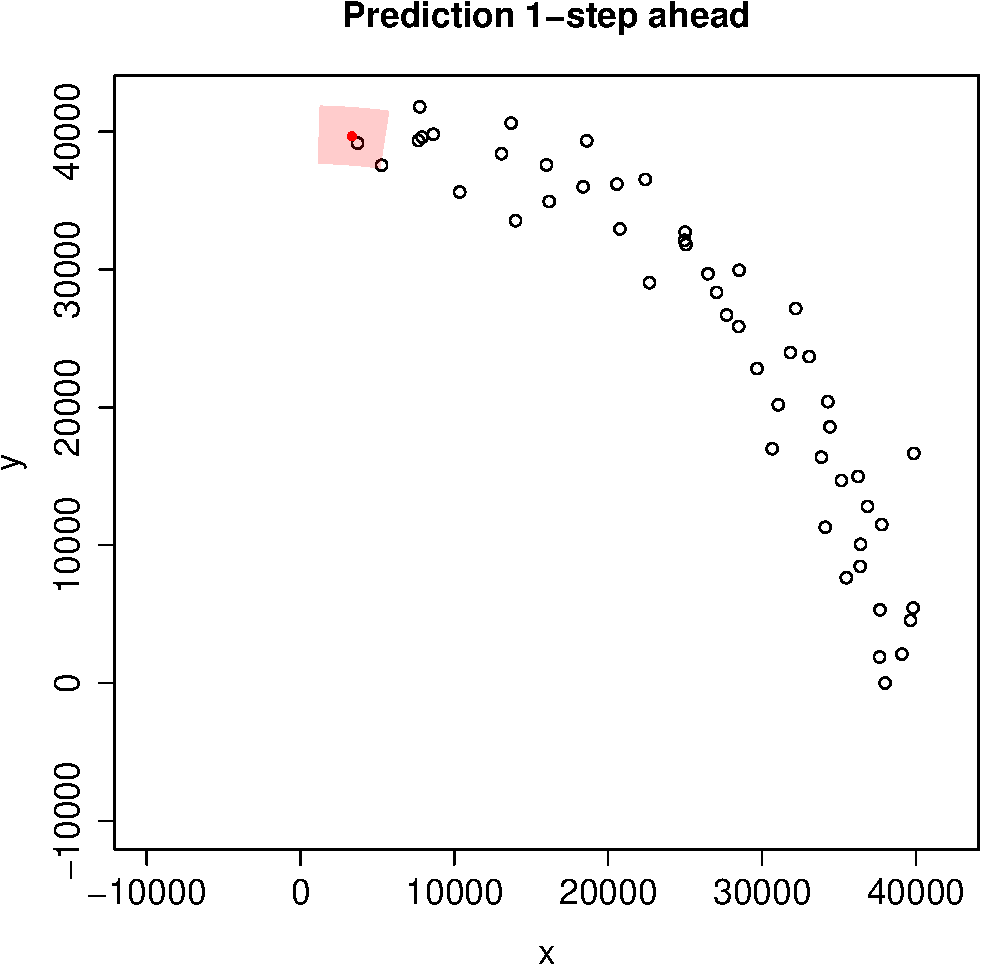
\includegraphics[width=70mm]{../plots/prediction-1.pdf}} \quad 
            \subfigure{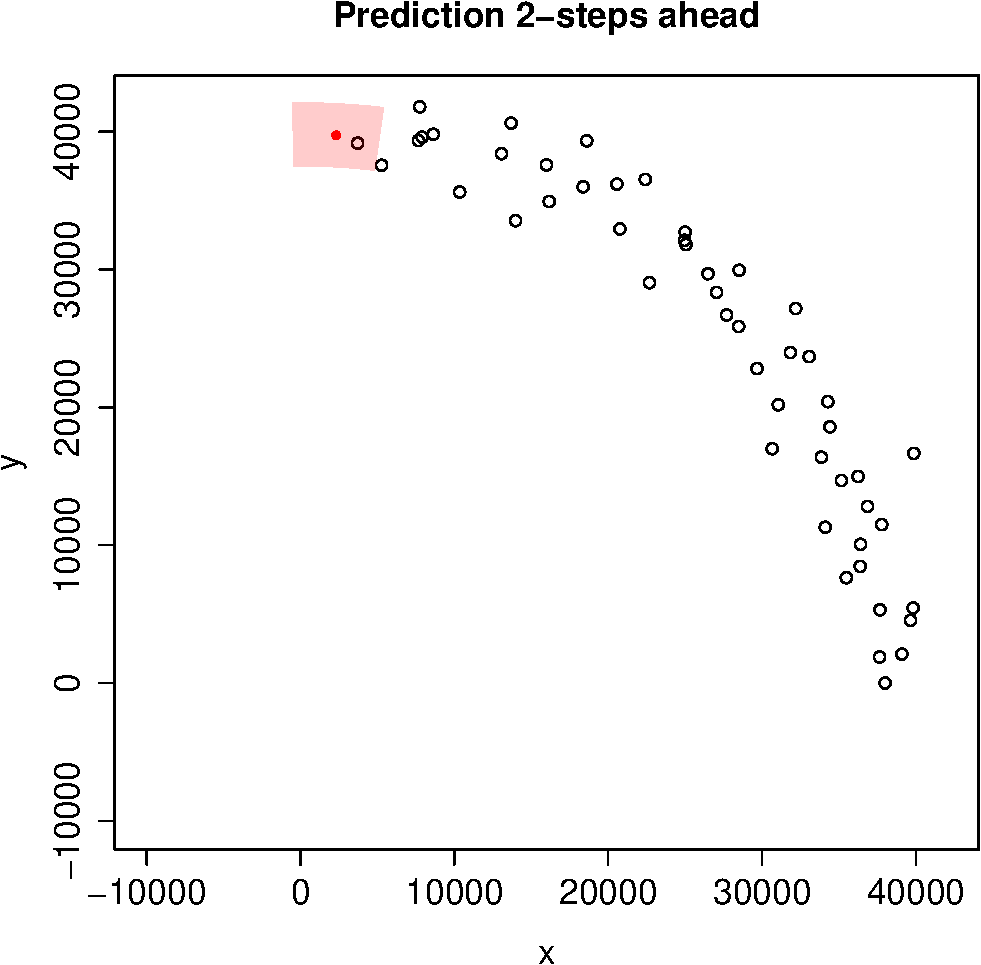
\includegraphics[width=70mm]{../plots/prediction-2.pdf}}}
    \mbox{\subfigure{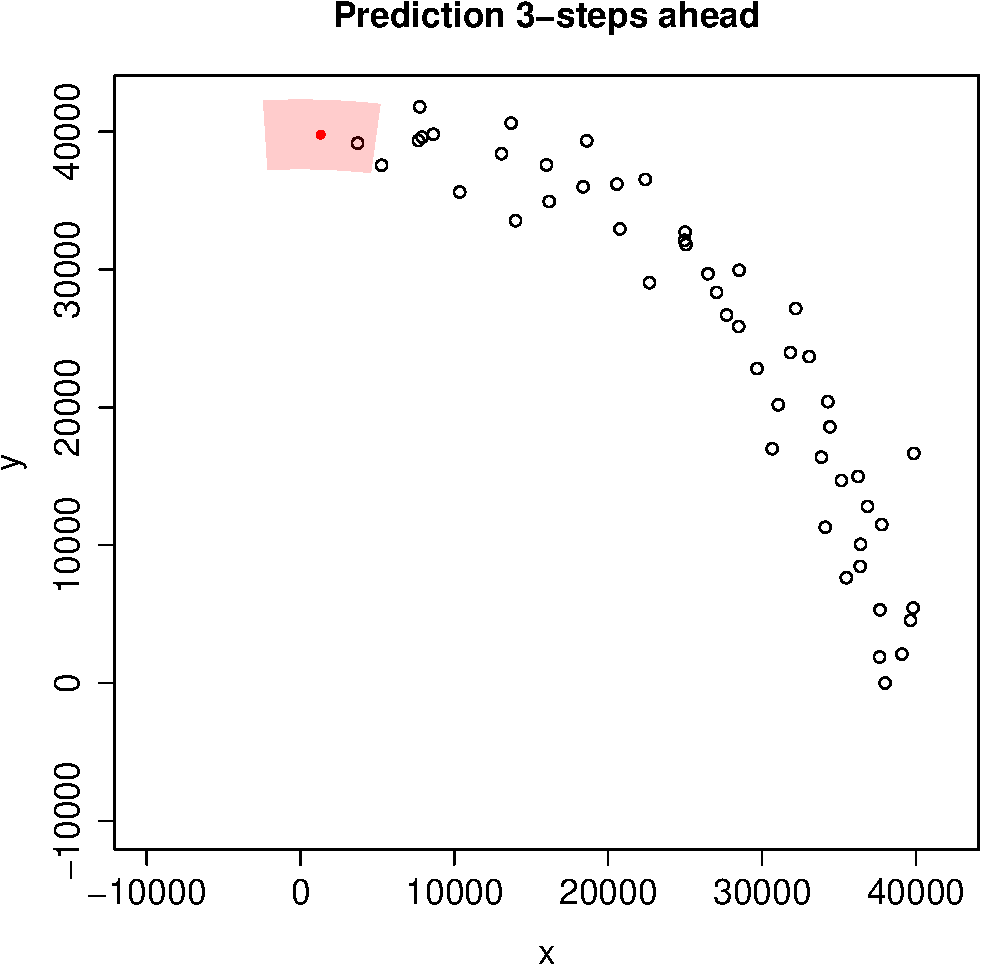
\includegraphics[width=70mm]{../plots/prediction-3.pdf}} \quad 
            \subfigure{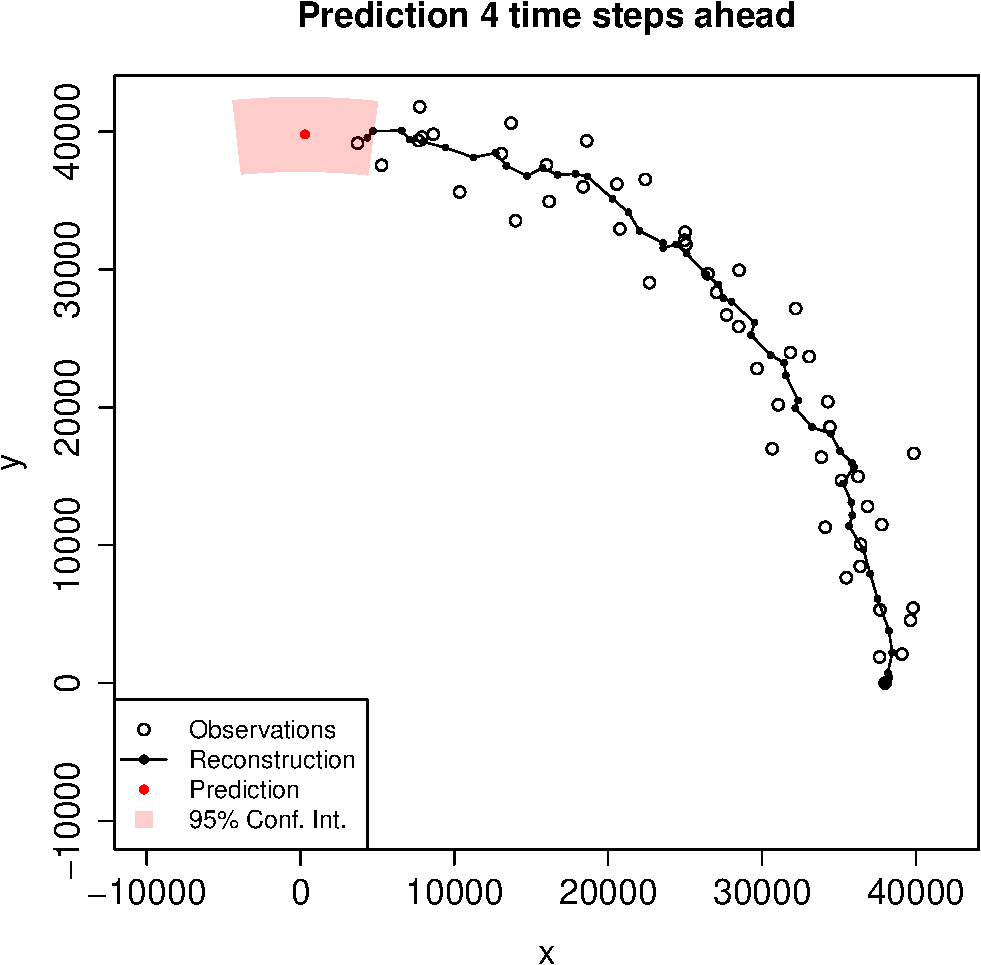
\includegraphics[width=70mm]{../plots/prediction-4.pdf}}}
    \mbox{\subfigure{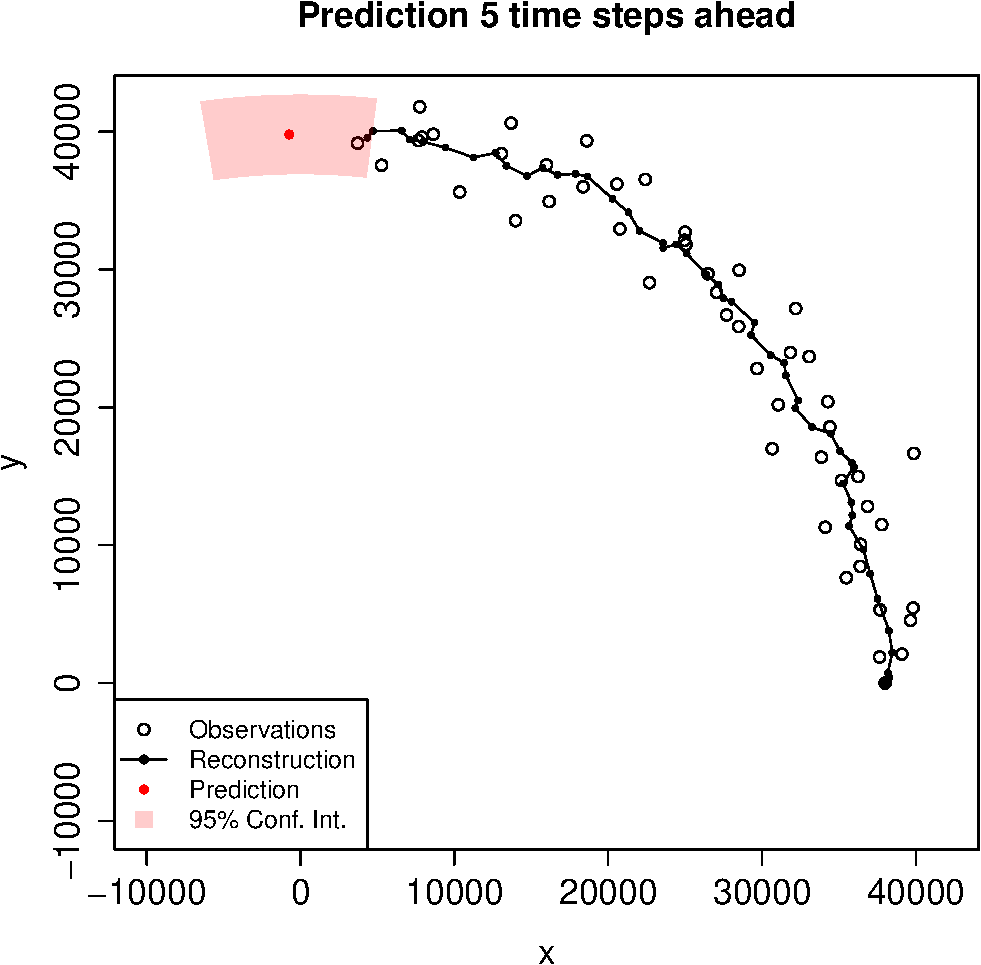
\includegraphics[width=70mm]{../plots/prediction-5.pdf}} \quad 
            \subfigure{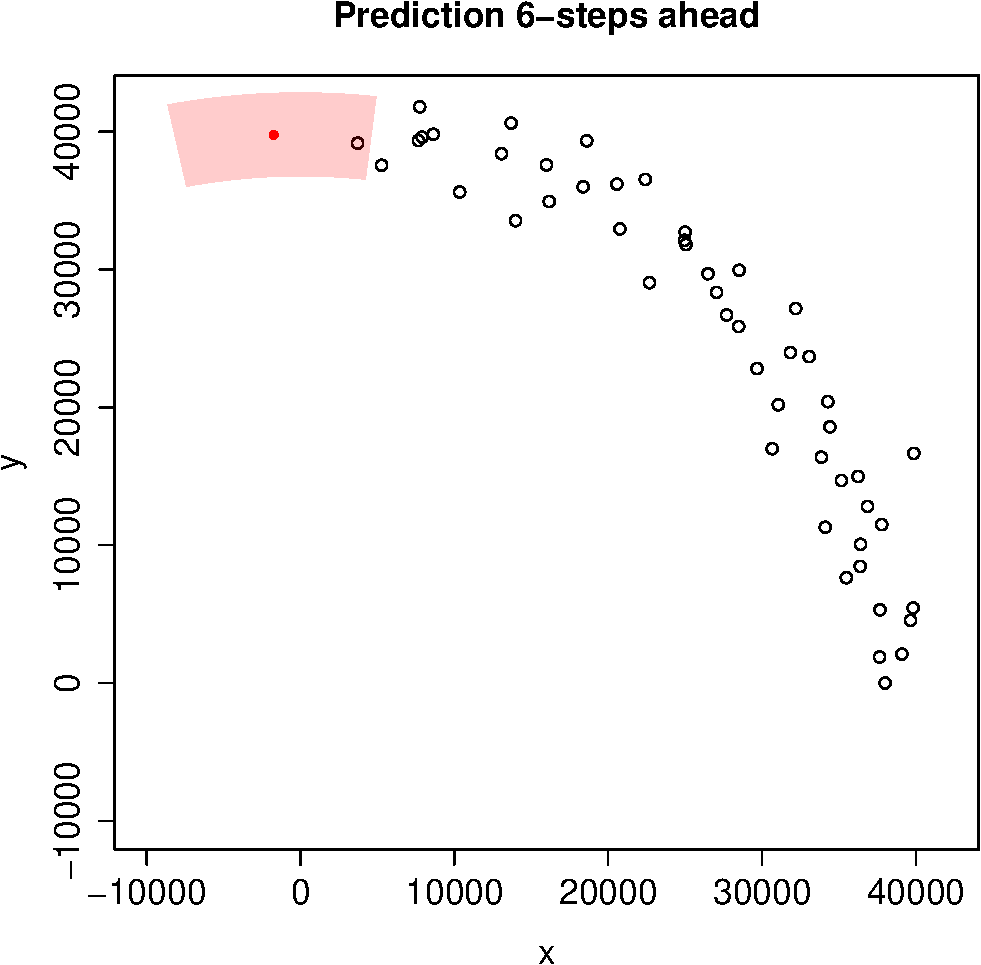
\includegraphics[width=70mm]{../plots/prediction-6.pdf}}}
    \caption{CAPTION}
    \label{fig:label}
\end{figure}

\FloatBarrier

\pagebreak

\renewcommand\thesection{\Alph{section}}
\section{Appendices}

All R code used for this assignment is included here. All source code incl.
latex code for this report can be found at \githuburl

%\subsection{Load data script}
%\lstinputlisting{../src/loaddata.R}

\pagebreak

\begin{thebibliography}{9}

\bibitem{hm}
  Henrik Madsen,
  \emph{Time Series Analysis}.
  Chapman \& Hall/CRC,
  1st Edition,
  2008.

%\bibitem{taleb}
%  Nassim Nicholas Taleb,
%  \emph{The Black Swan}.
%  Random House Trade Paperbacks
%  2nd Edition,
%  2010.

\end{thebibliography}


\end{document}
